\begin{figure}[htbp]
\centering
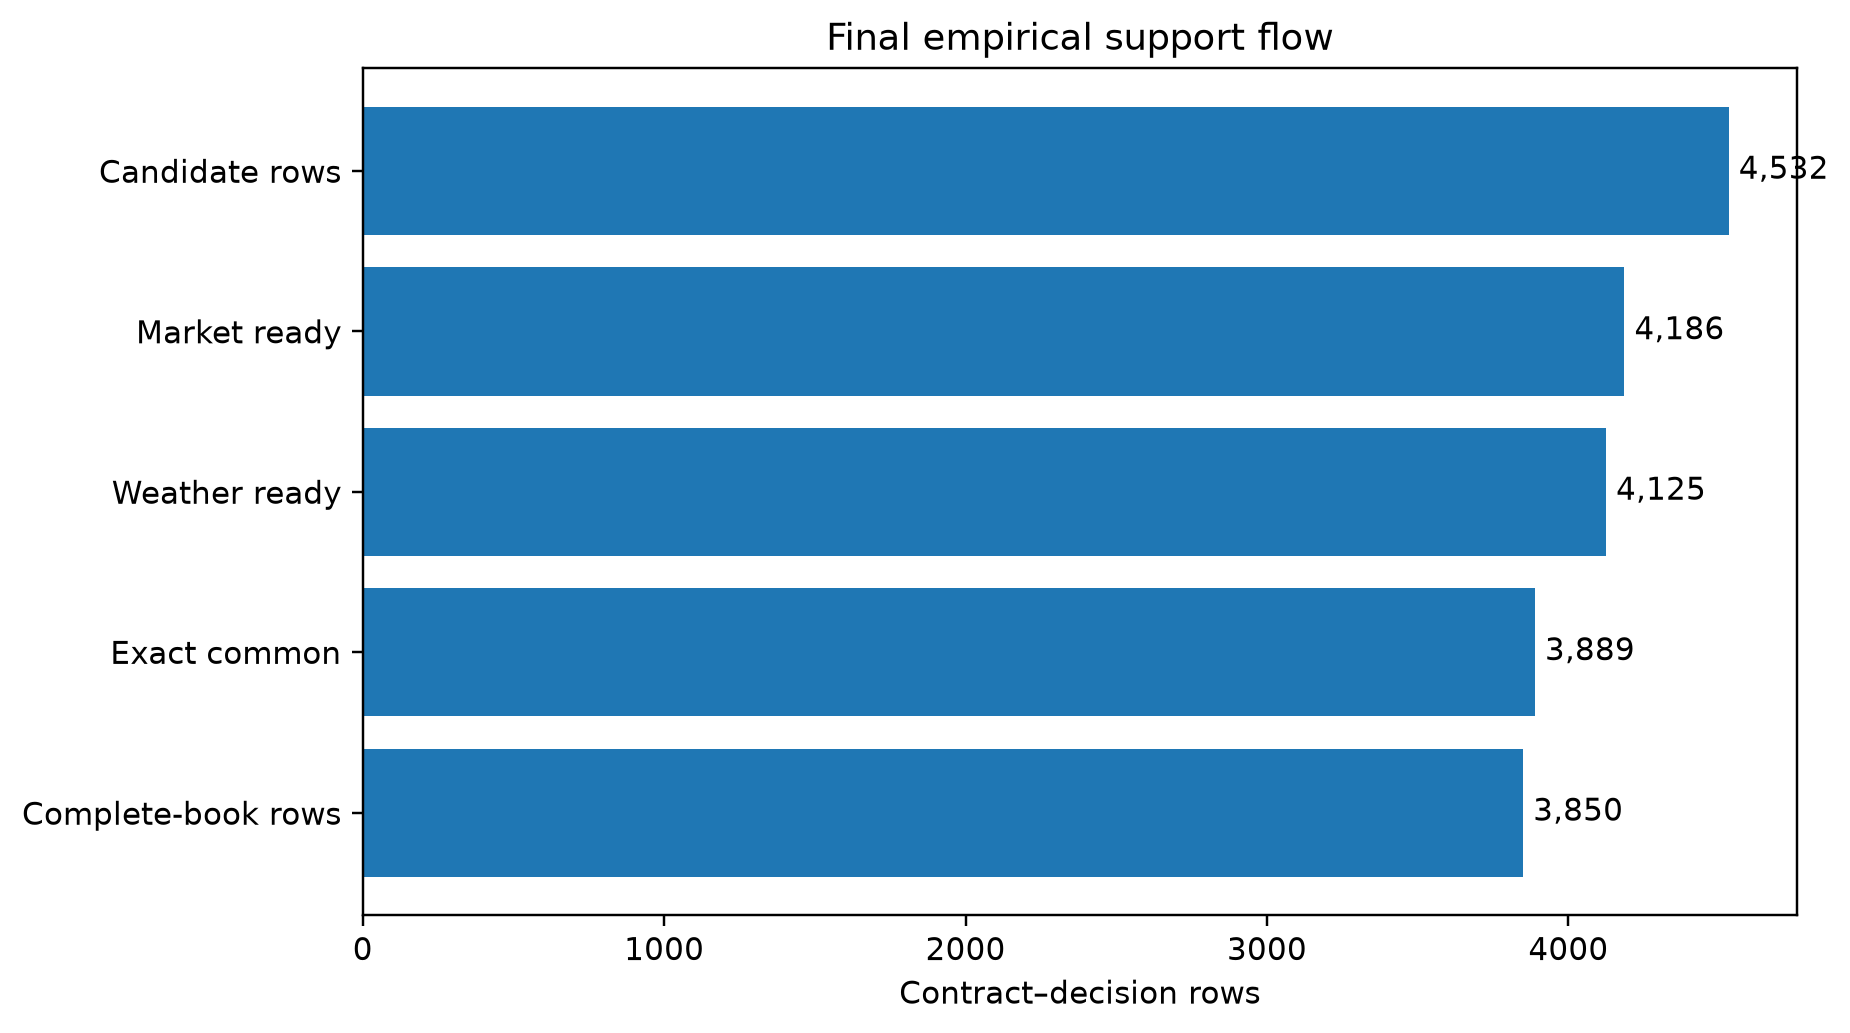
\includegraphics[width=0.92\textwidth]{figures/18yB_sample_support_flow.png}
\caption{Final empirical support flow from candidate rows to complete-book contract rows.}
\label{fig:sample_support_flow}
\end{figure}

\begin{figure}[htbp]
\centering
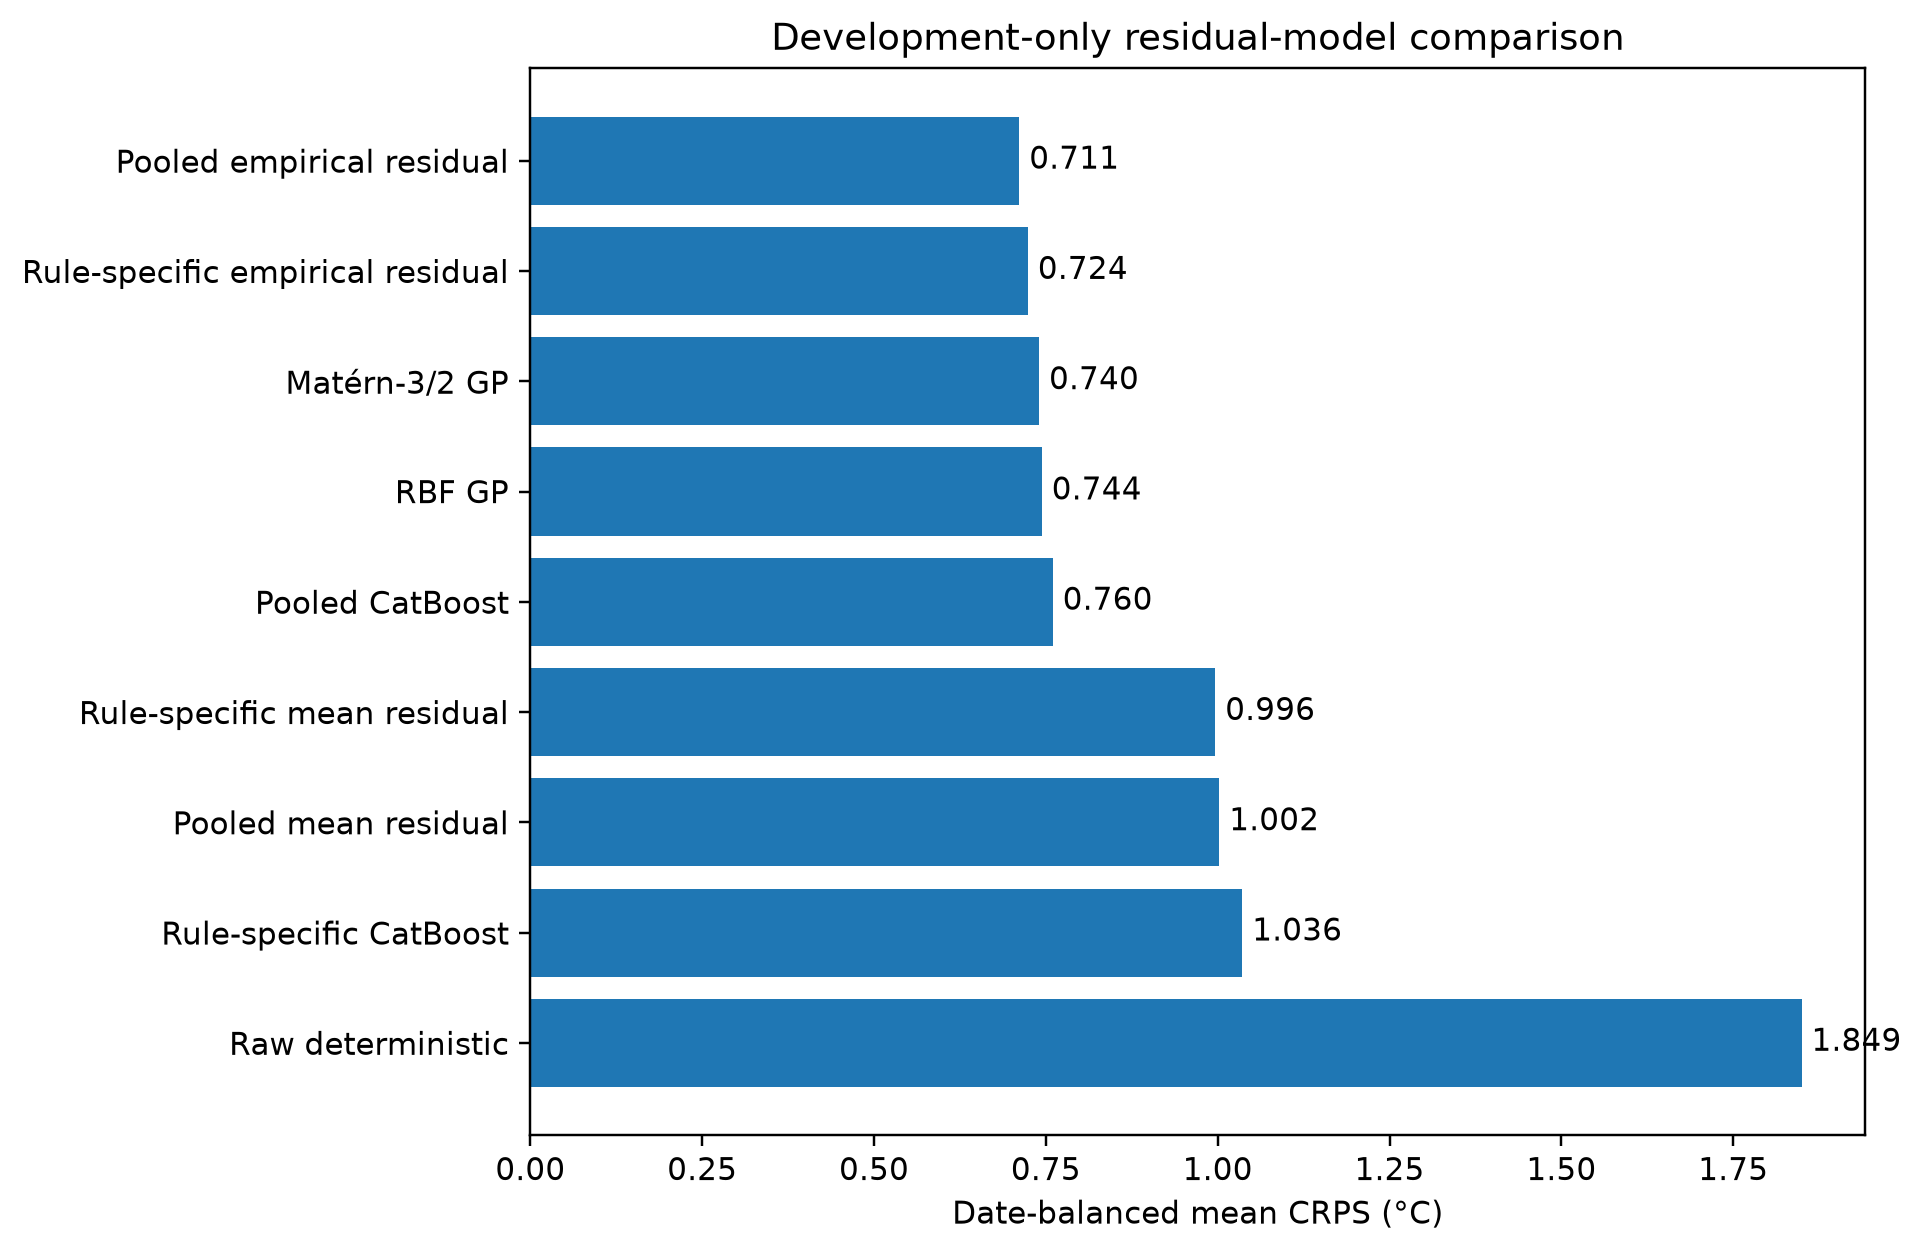
\includegraphics[width=0.92\textwidth]{figures/18yB_development_crps.png}
\caption{Development-only CRPS comparison for all nine frozen candidates.}
\label{fig:development_crps}
\end{figure}

\begin{figure}[htbp]
\centering
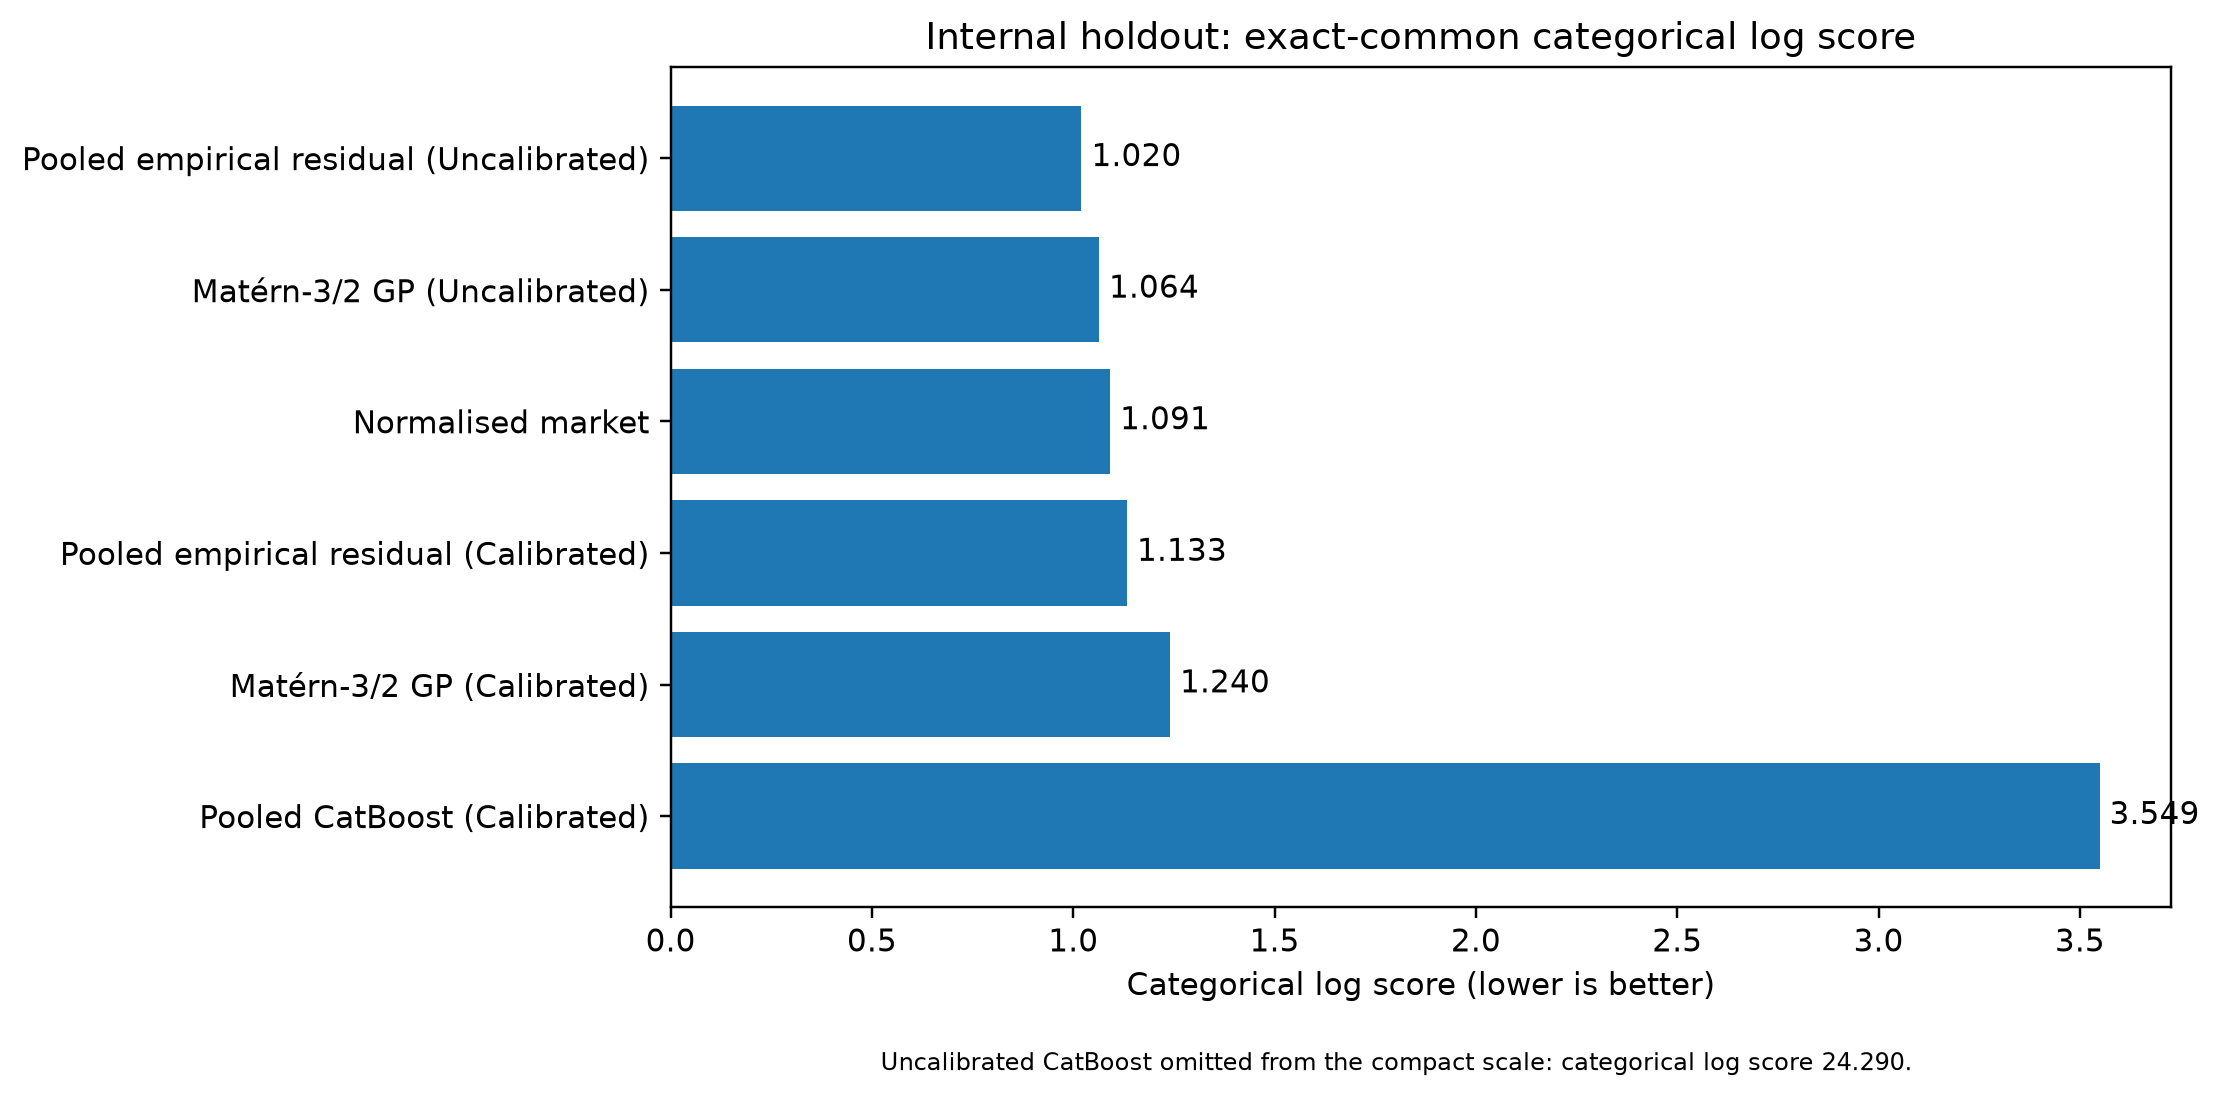
\includegraphics[width=0.92\textwidth]{figures/18yB_holdout_probability_log.png}
\caption{Exact-common categorical log scores on the locked internal holdout. The uncalibrated CatBoost value 24.290 is omitted from the compact scale and retained in the full audit table.}
\label{fig:holdout_probability_log}
\end{figure}

\begin{figure}[htbp]
\centering
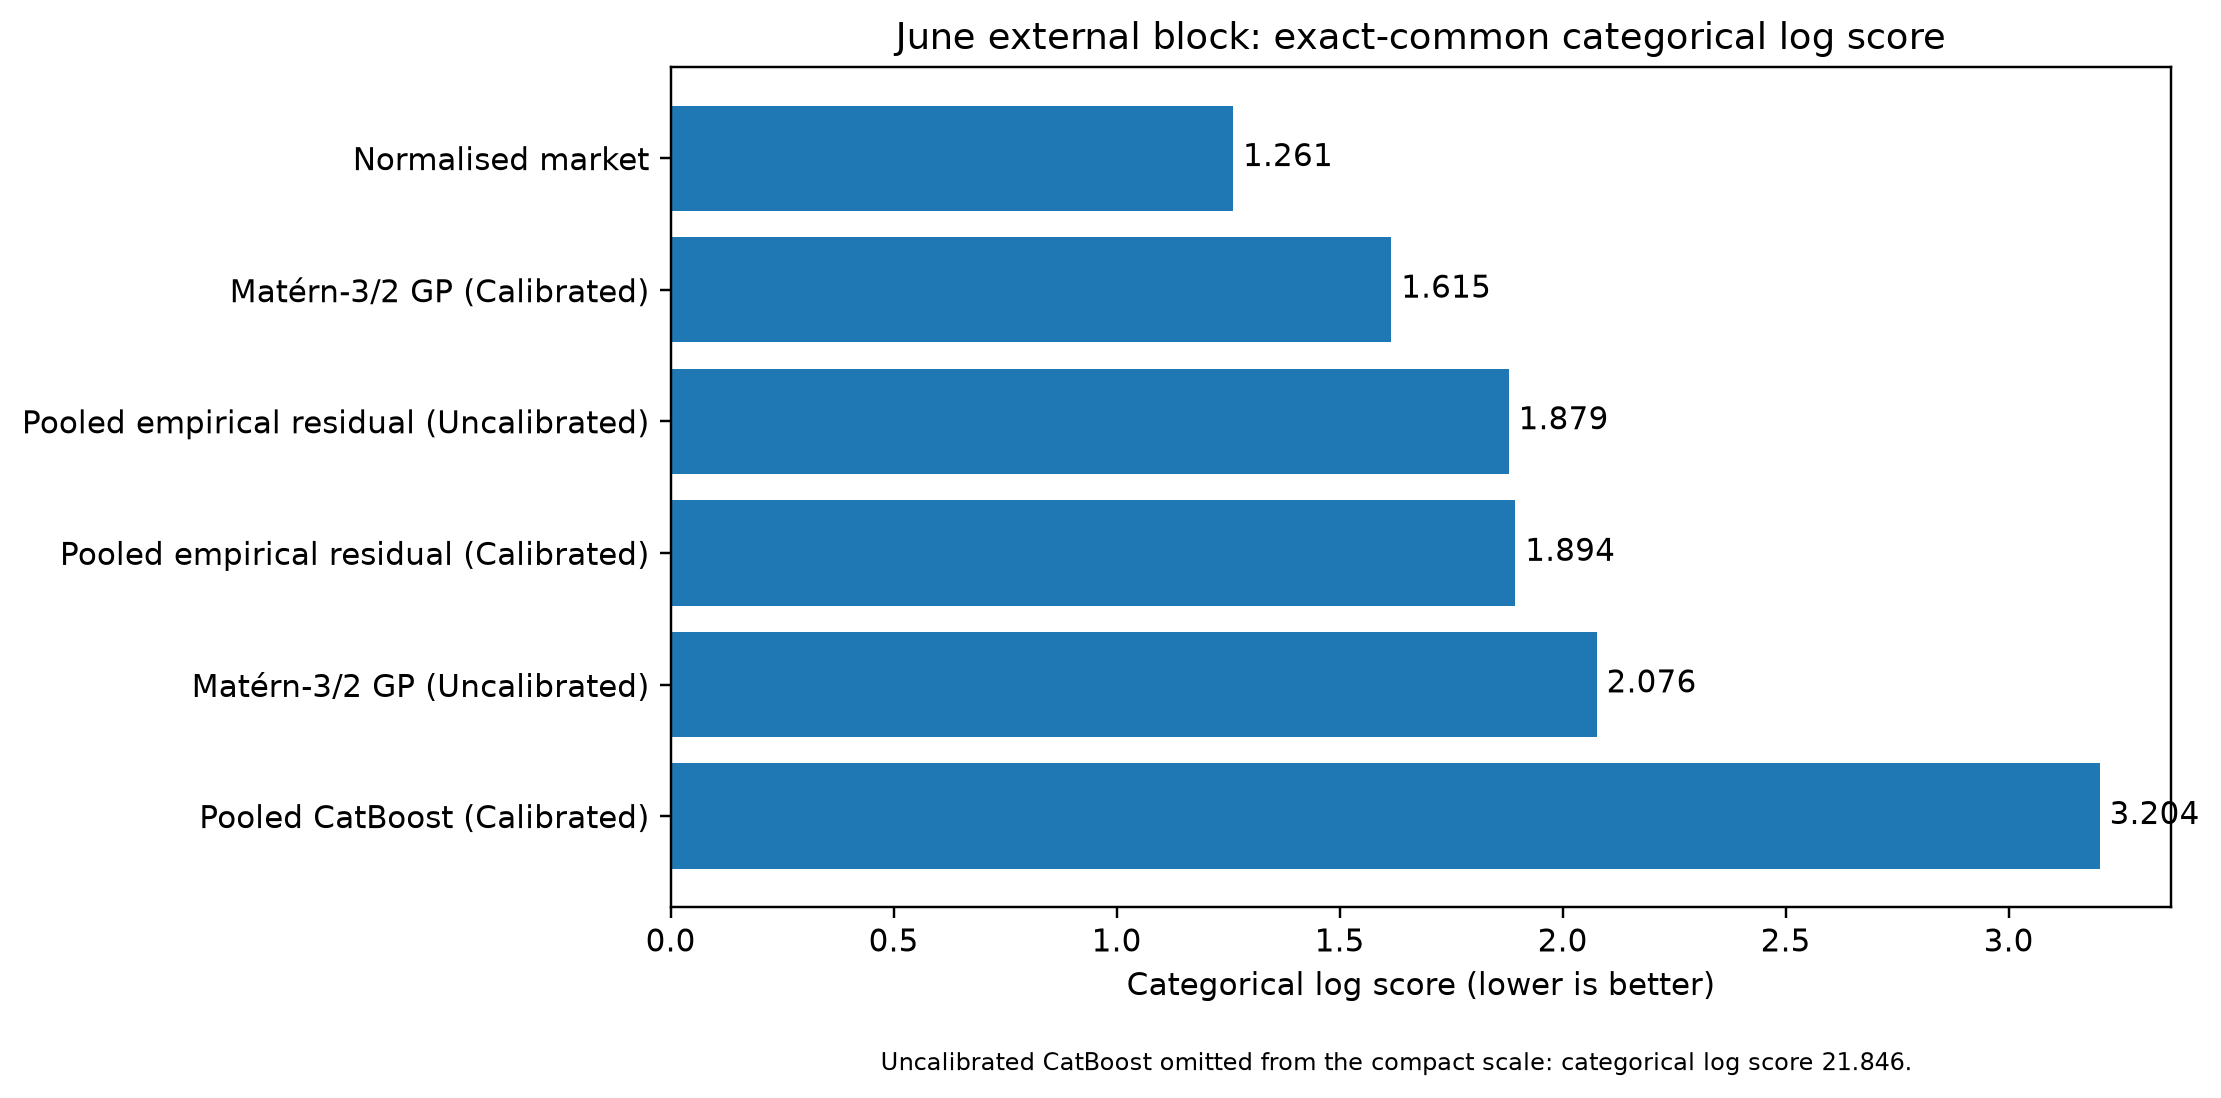
\includegraphics[width=0.92\textwidth]{figures/18yB_external_probability_log.png}
\caption{Exact-common categorical log scores on the June external block. The uncalibrated CatBoost value 21.846 is omitted from the compact scale and retained in the full audit table.}
\label{fig:external_probability_log}
\end{figure}

\begin{figure}[htbp]
\centering
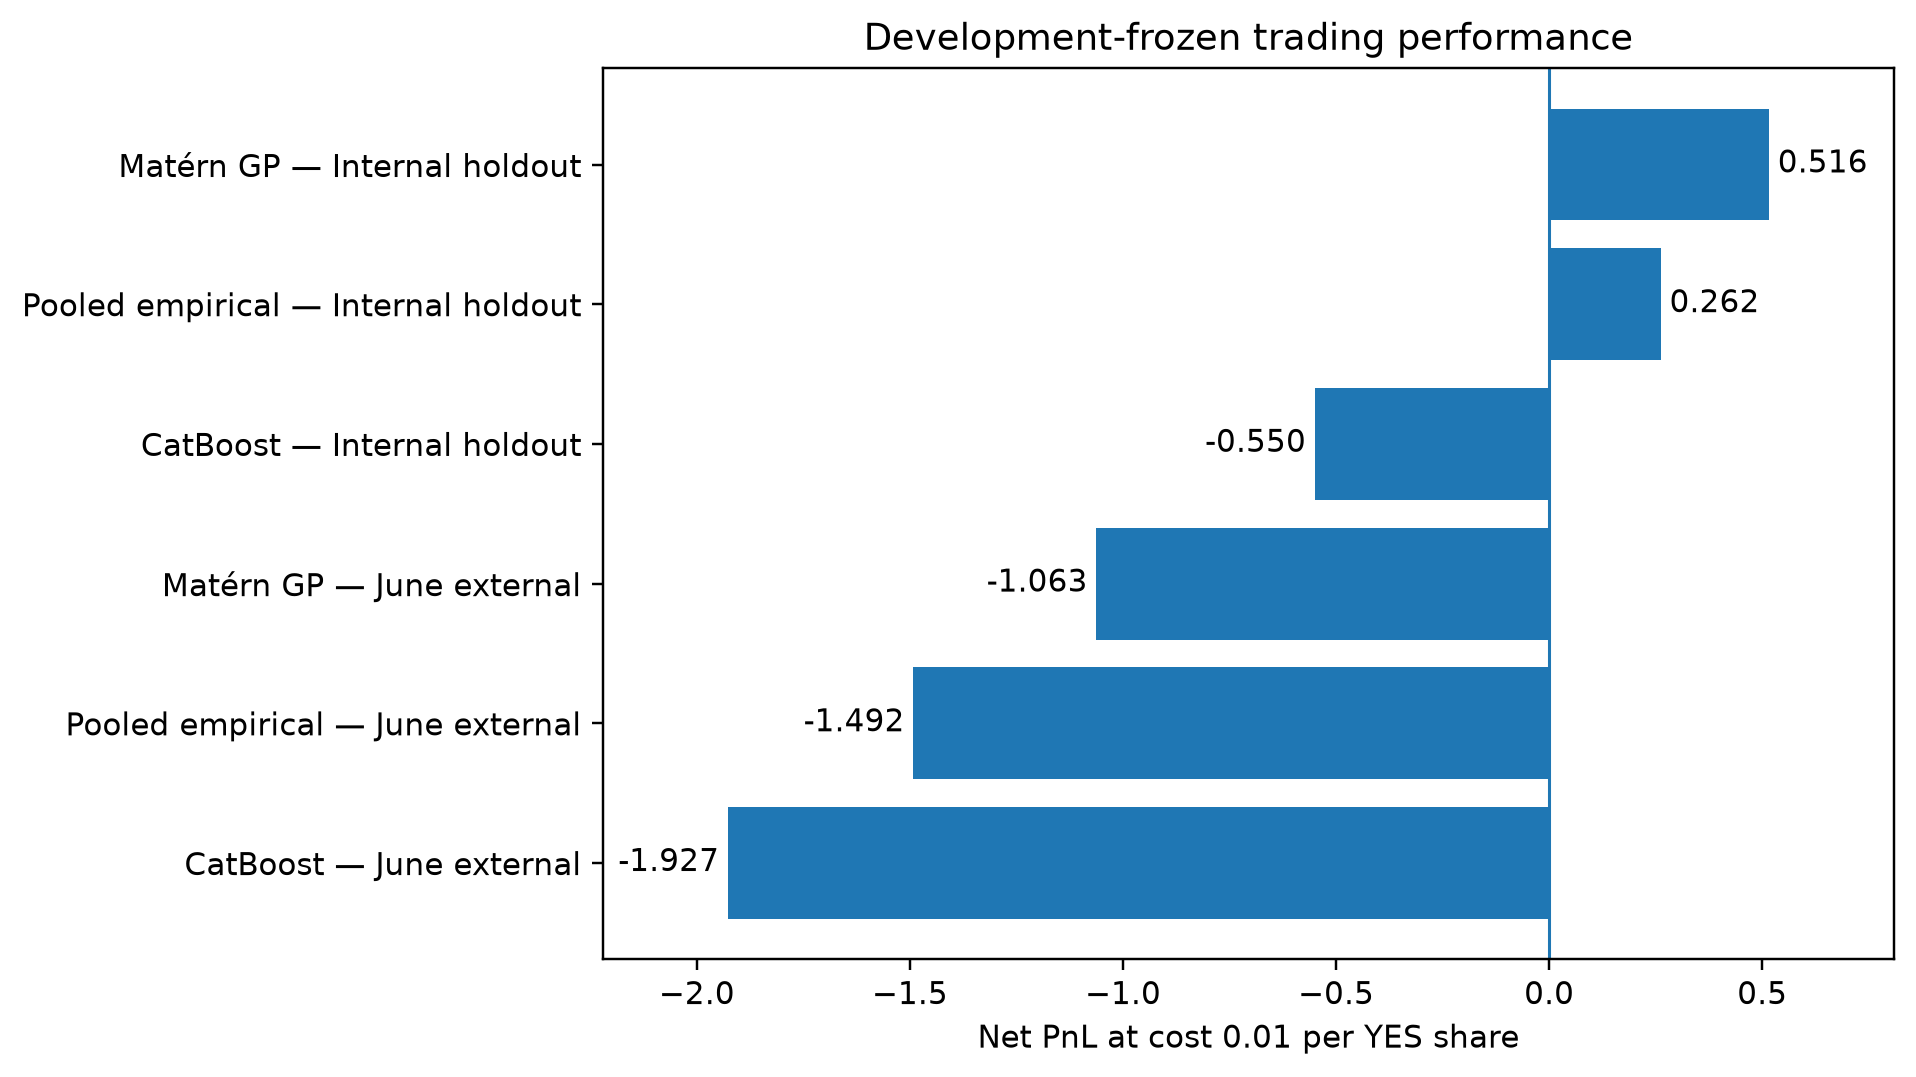
\includegraphics[width=0.92\textwidth]{figures/18yB_trading_net_pnl.png}
\caption{Net PnL of the three development-frozen strategies on the holdout and June blocks.}
\label{fig:trading_net_pnl}
\end{figure}

\begin{figure}[htbp]
\centering
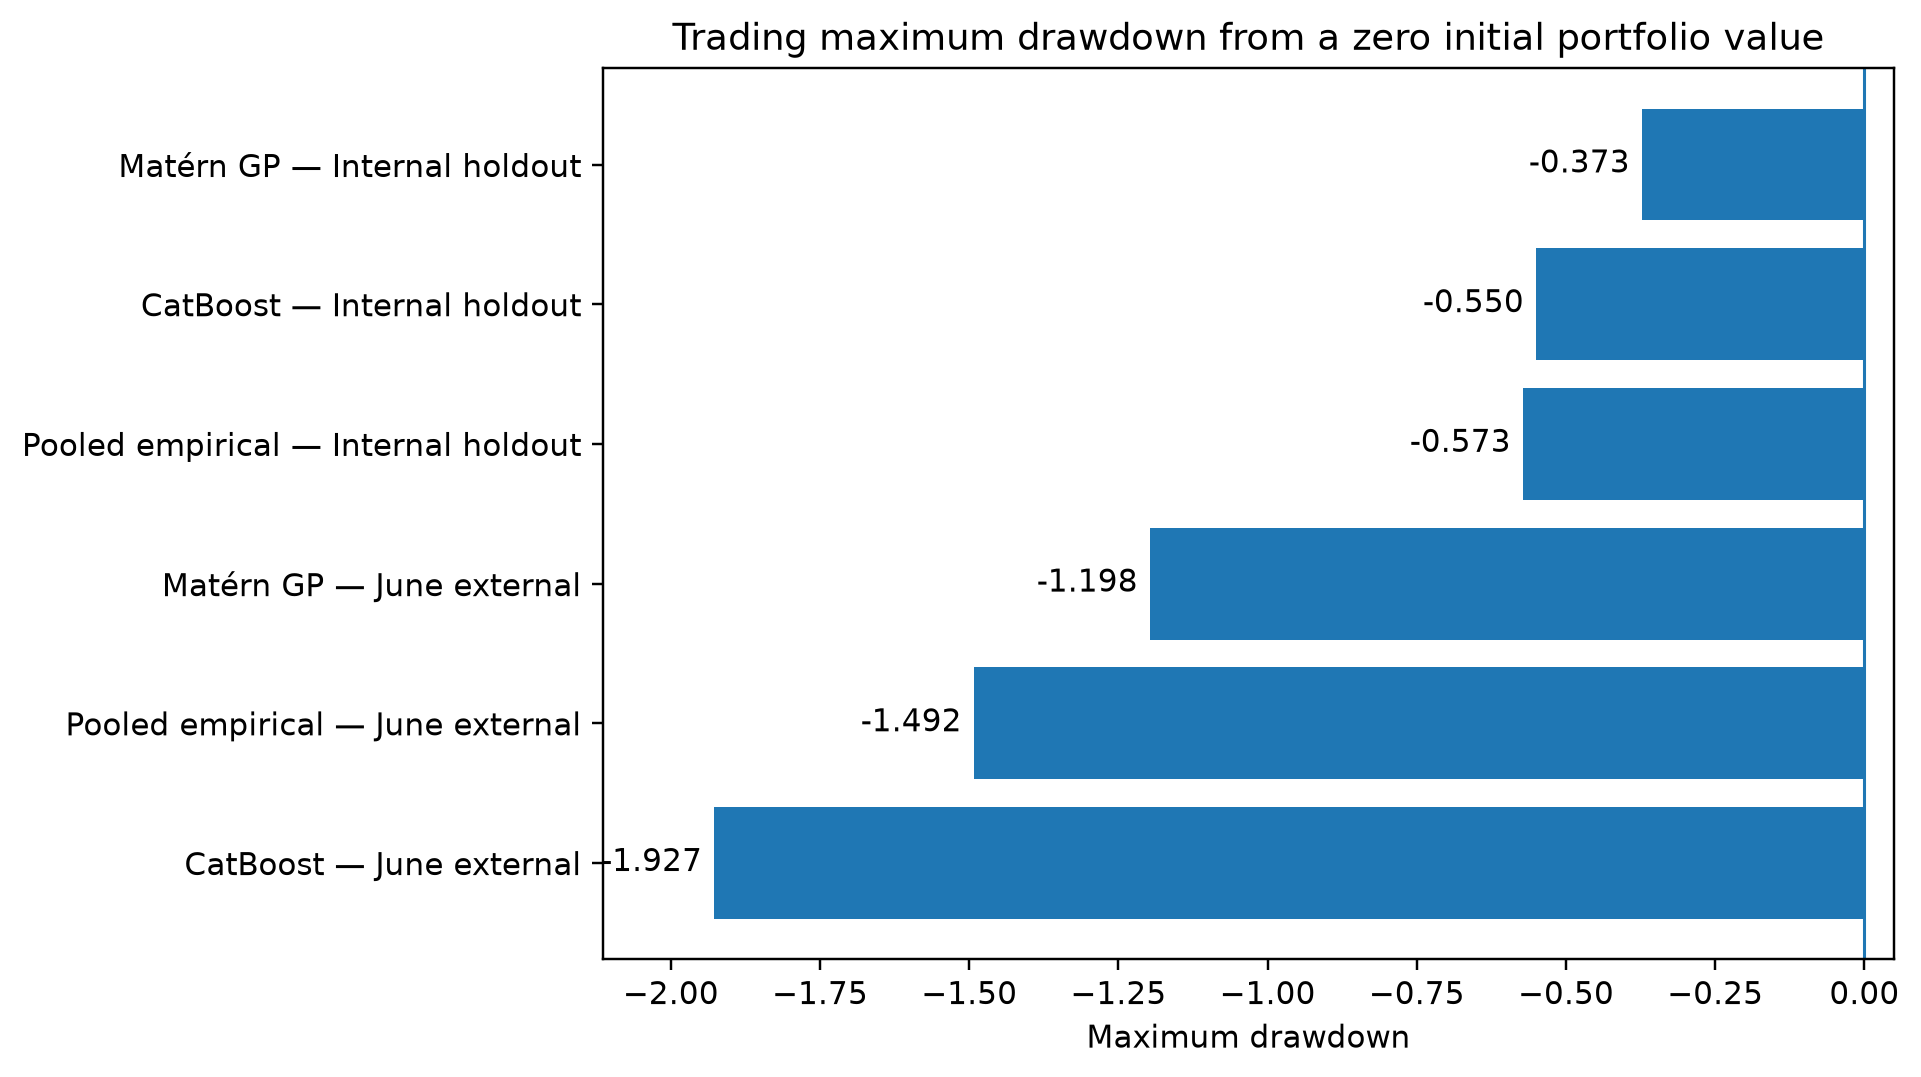
\includegraphics[width=0.92\textwidth]{figures/18yB_trading_maximum_drawdown.png}
\caption{Maximum drawdown for the three development-frozen strategies, including the zero initial portfolio value.}
\label{fig:trading_maximum_drawdown}
\end{figure}
